% move all configuration stuff into one file so we can focus on the content
\documentclass[aspectratio=169,hyperref={pdfpagelabels=false,colorlinks=true,linkcolor=white,urlcolor=lightblue},xcolor={table},t]{beamer}

%%%%%%%%%%%%%%%%%%%%%%%%%%%%%%%%%%%%%%%%%%%%%%%%%%%%%%%%%%%%%%%%%%%%%%%%%%%%%%%%%%
%%%%%%%%%%%%%%%%%%%%%%%%%%%%%%%%%%%%%%%%%%%%%%%%%%%%%%%%%%%%%%%%%%%%%%%%%%%%%%%%%%
% packages
\usepackage{pict2e}
\usepackage{epic}
\usepackage{amsmath,amsfonts,amssymb}
\usepackage{units}
\usepackage{fancybox}
\usepackage[absolute,overlay]{textpos} 
%\usepackage[table]{xcolor}
\usepackage{animate}
\usepackage{gensymb}
%\usepackage{graphicx}
%\usepackage{longtable}
\usepackage{multirow}
\usepackage{silence}
\usepackage{tikz}
\usepackage[backend=bibtex,style=ieee]{biblatex}
\AtEveryCitekey{\iffootnote{\tiny}{}}
%\addbibresource{include/references}



% fontsize
\let\Tiny=\tiny

%%%%%%%%%%%%%%%%%%%%%%%%%%%%%%%%%%%%%%%%%%%%%%%%%%%%%%%%%%%%%%%%%%%%%%%%%%%%%%%%%%
%%%%%%%%%%%%%%%%%%%%%%%%%%%%%%%%%%%%%%%%%%%%%%%%%%%%%%%%%%%%%%%%%%%%%%%%%%%%%%%%%%
% warnings
\pdfsuppresswarningpagegroup=1
\WarningFilter{biblatex}{Patching footnotes failed}
\WarningFilter{latexfont}{Font shape}
\WarningFilter{latexfont}{Some font shapes}
\WarningFilter{gensymb}{Not defining}


%%%%%%%%%%%%%%%%%%%%%%%%%%%%%%%%%%%%%%%%%%%%%%%%%%%%%%%%%%%%%%%%%%%%%%%%%%%%%%%%%%
%%%%%%%%%%%%%%%%%%%%%%%%%%%%%%%%%%%%%%%%%%%%%%%%%%%%%%%%%%%%%%%%%%%%%%%%%%%%%%%%%%
% theme & layout
\usetheme{Frankfurt}
\useinnertheme{rectangles}


%%%%%%%%%%%%%%%%%%%%%%%%%%%%%%%%%%%%%%%%%%%%%%%%%%%%%%%%%%%%%%%%%%%%%%%%%%%%%%%%%%
\setbeamertemplate{frametitle}[default][colsep=-4bp,rounded=false,shadow=false]
\setbeamertemplate{frametitle}
{%
    \nointerlineskip%
    %\vskip-0.5ex
    \begin{beamercolorbox}[wd=\paperwidth,ht=3.5ex,dp=0.6ex]{frametitle}
        \hspace*{1.3ex}\insertframetitle%
        
        \hspace*{1.3ex}\small\insertframesubtitle%
    \end{beamercolorbox}%
    \begin{textblock*}{100mm}(13.75cm,1cm)
        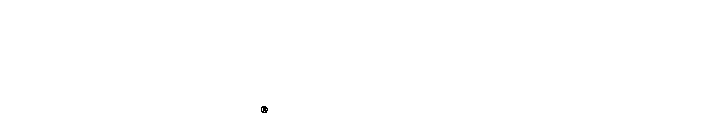
\includegraphics[height=.4cm,keepaspectratio]{../shared/Logo_GTCMT_white}
    \end{textblock*}
}


%%%%%%%%%%%%%%%%%%%%%%%%%%%%%%%%%%%%%%%%%%%%%%%%%%%%%%%%%%%%%%%%%%%%%%%%%%%%%%%%%%
\setbeamertemplate{title page}[default][colsep=-4bp,rounded=false,shadow=false]
\setbeamertemplate{title page}
{
    %\begin{textblock*}{100mm}(15cm,.51cm)
            %\href{https://github.com/alexanderlerch/ACA-Slides/blob/2nd_edition/\jobname.pdf}{\includegraphics[height=.5cm,keepaspectratio]{graph/Logo_github}}\hspace*{2ex}
    %\end{textblock*}
    %\begin{textblock*}{100mm}(15cm,1.3cm)
            %\href{\IEEELink}{\includegraphics[height=.5cm,keepaspectratio]{graph/icon/book}}\hspace*{2ex}
    %\end{textblock*}
    \vskip-10ex
    \begin{beamercolorbox}[wd=\paperwidth,ht=.7\paperheight,dp=0.6ex]{frametitle} %35ex
        %\begin{flushright}
            %\href{http://www.gtcmt.gatech.edu}{
\includegraphics[height=.8cm,keepaspectratio]{graph/Logo_GTCMT_black}}\hspace*{2ex}
        %\end{flushright}
        
        \hspace*{1.8ex}\LARGE\inserttitle%
        
        \vspace*{.5ex}
        
        \hspace*{1.3ex}\small\insertsubtitle%
        
        \vspace*{.5ex}
    \end{beamercolorbox}%
    \nointerlineskip%
    \begin{beamercolorbox}[wd=\paperwidth,ht=.4\paperheight,dp=0.6ex]{page number in head/foot}
        %\vspace*{-.5ex}
        \hspace*{1.7ex}\small\insertauthor%
        
        %\hspace*{1.7ex}\small }%
        
        \vspace*{12ex}
        \vfill
        \begin{flushright}
            \href{http://www.gtcmt.gatech.edu}{
\includegraphics[height=.5cm,keepaspectratio]{../shared/Logo_GTCMT_black}}\hspace*{2ex}
        \end{flushright}
    \end{beamercolorbox}%
}


%%%%%%%%%%%%%%%%%%%%%%%%%%%%%%%%%%%%%%%%%%%%%%%%%%%%%%%%%%%%%%%%%%%%%%%%%%%%%%%%%%
%\makeatother
\setbeamertemplate{footline}
{
  \leavevmode%
  \hbox{%
  \begin{beamercolorbox}[wd=.5\paperwidth,ht=2.25ex,dp=1ex,left,leftskip=1ex]{page number in head/foot}%
    \insertsubtitle
  \end{beamercolorbox}%
  \begin{beamercolorbox}[wd=.5\paperwidth,ht=2.25ex,dp=1ex,right,rightskip=1ex]{page number in head/foot}%
    \hfill
    \insertframenumber{} / \inserttotalframenumber
  \end{beamercolorbox}}%
  \vskip0pt%
}
%\makeatletter


%%%%%%%%%%%%%%%%%%%%%%%%%%%%%%%%%%%%%%%%%%%%%%%%%%%%%%%%%%%%%%%%%%%%%%%%%%%%%%%%%%
\beamertemplatenavigationsymbolsempty
\setbeamertemplate{navigation symbols}{}
\setbeamertemplate{blocks}[default]%[rounded=false,shadow=false]
\setbeamertemplate{itemize item}[square]
\setbeamertemplate{itemize subitem}[circle]
\setbeamertemplate{itemize subsubitem}[triangle]
\setbeamertemplate{enumerate item}[square]
\setbeamertemplate{enumerate subitem}[circle]
\setbeamertemplate{enumerate subsubitem}[circle]


%%%%%%%%%%%%%%%%%%%%%%%%%%%%%%%%%%%%%%%%%%%%%%%%%%%%%%%%%%%%%%%%%%%%%%%%%%%%%%%%%%
% colors
\setbeamercolor{structure}{fg=darkgray}
\setbeamercovered{transparent} %invisible
\setbeamercolor{bibliography entry author}{fg=black}
\setbeamercolor*{bibliography entry title}{fg=black}
\setbeamercolor*{bibliography entry note}{fg=black}
\setbeamercolor{frametitle}{fg=black}
\setbeamercolor{title}{fg=white}
\setbeamercolor{subtitle}{fg=white}
\setbeamercolor{frametitle}{fg=white}
\setbeamercolor{framesubtitle}{fg=white}
\setbeamercolor{mini frame}{fg=white, bg=black}
\setbeamercolor{section in head/foot}{fg=white, bg=darkgray}
\setbeamercolor{page number in head/foot}{fg=black, bg=gtgold}
\setbeamercolor{item projected}{fg=white, bg=black}

%---------------------------------------------------------------------------------

%%%%%%%%%%%%%%%%%%%%%%%%%%%%%%%%%%%%%%%%%%%%%%%%%%%%%%%%%%%%%%%%%%%%%%%%%%%%%%%%%%
%%%%%%%%%%%%%%%%%%%%%%%%%%%%%%%%%%%%%%%%%%%%%%%%%%%%%%%%%%%%%%%%%%%%%%%%%%%%%%%%%%
% title information
\title[]{MUSI6202: Digital Signal Processing for Music}   
\author[alexander lerch]{alexander lerch} 
%\institute{~}
%\date[Alexander Lerch]{}
%\titlegraphic{\vspace{-16mm}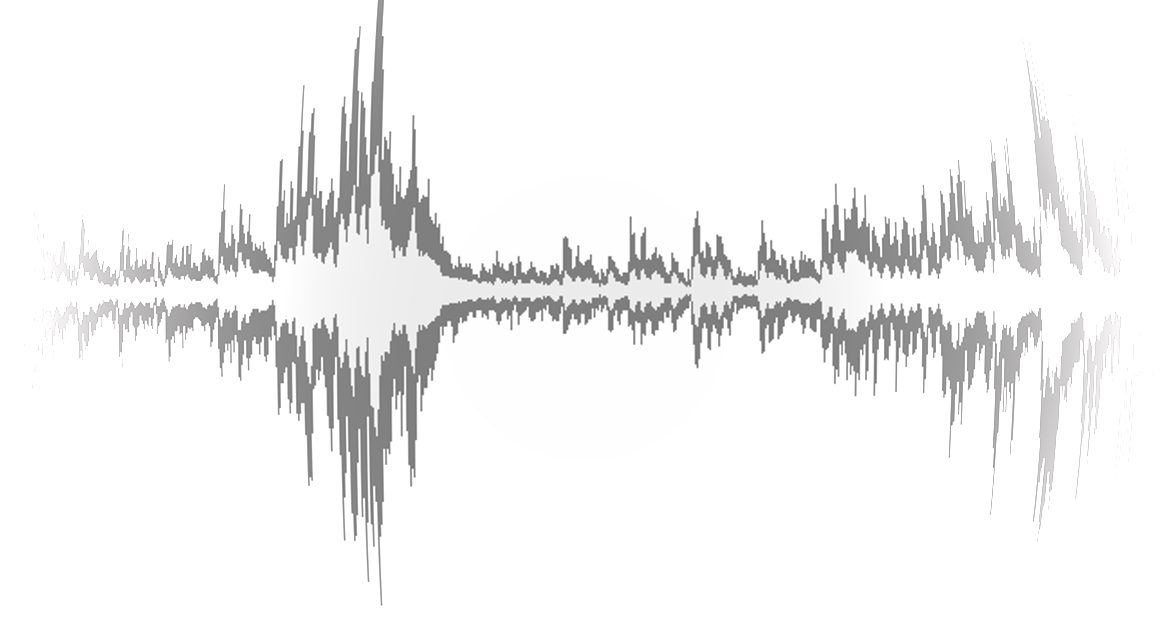
\includegraphics[width=\textwidth,height=3cm]{title}}

%%%%%%%%%%%%%%%%%%%%%%%%%%%%%%%%%%%%%%%%%%%%%%%%%%%%%%%%%%%%%%%%%%%%%%%%%%%%%%%%%%
%%%%%%%%%%%%%%%%%%%%%%%%%%%%%%%%%%%%%%%%%%%%%%%%%%%%%%%%%%%%%%%%%%%%%%%%%%%%%%%%%%
% colors
\definecolor{gtgold}{rgb}{.914, .664, 0} %0e7eed {rgb}{0.88,0.66,1,0.06} [234, 170, 0]/256 %96caff
\definecolor{darkgray}{rgb}{.15, .15, .15}
\definecolor{lightblue}{HTML}{0e7eed}
\definecolor{highlight}{rgb}{0, 0, 1} %_less!40

%%%%%%%%%%%%%%%%%%%%%%%%%%%%%%%%%%%%%%%%%%%%%%%%%%%%%%%%%%%%%%%%%%%%%%%%%%%%%%%%%%
%%%%%%%%%%%%%%%%%%%%%%%%%%%%%%%%%%%%%%%%%%%%%%%%%%%%%%%%%%%%%%%%%%%%%%%%%%%%%%%%%%
% relative paths
\graphicspath{{../graph/}}


%%%%%%%%%%%%%%%%%%%%%%%%%%%%%%%%%%%%%%%%%%%%%%%%%%%%%%%%%%%%%%%%%%%%%%%%%%%%%%%%%%
%%%%%%%%%%%%%%%%%%%%%%%%%%%%%%%%%%%%%%%%%%%%%%%%%%%%%%%%%%%%%%%%%%%%%%%%%%%%%%%%%%
% units
\setlength{\unitlength}{1mm}

%%%%%%%%%%%%%%%%%%%%%%%%%%%%%%%%%%%%%%%%%%%%%%%%%%%%%%%%%%%%%%%%%%%%%%%%%%%%%%%%%%
%%%%%%%%%%%%%%%%%%%%%%%%%%%%%%%%%%%%%%%%%%%%%%%%%%%%%%%%%%%%%%%%%%%%%%%%%%%%%%%%%%
% math
\DeclareMathOperator*{\argmax}{argmax}
\DeclareMathOperator*{\argmin}{argmin}
\DeclareMathOperator*{\atan}{atan}
\DeclareMathOperator*{\arcsinh}{arcsinh}
\DeclareMathOperator*{\sign}{sign}
\DeclareMathOperator*{\tcdf}{tcdf}
\DeclareMathOperator*{\si}{sinc}
\DeclareMathOperator*{\princarg}{princarg}
\DeclareMathOperator*{\arccosh}{arccosh}
\DeclareMathOperator*{\hwr}{HWR}
\DeclareMathOperator*{\flip}{flip}
\DeclareMathOperator*{\sinc}{sinc}
\DeclareMathOperator*{\floor}{floor}
\newcommand{\e}{{e}}
\newcommand{\jom}{\mathrm{j}\omega}
\newcommand{\jOm}{\mathrm{j}\Omega}
\newcommand   {\mat}[1]    		{\boldsymbol{\uppercase{#1}}}		%bold
\renewcommand {\vec}[1]    		{\boldsymbol{\lowercase{#1}}}		%bold

%%%%%%%%%%%%%%%%%%%%%%%%%%%%%%%%%%%%%%%%%%%%%%%%%%%%%%%%%%%%%%%%%%%%%%%%%%%%%%%%%%
%%%%%%%%%%%%%%%%%%%%%%%%%%%%%%%%%%%%%%%%%%%%%%%%%%%%%%%%%%%%%%%%%%%%%%%%%%%%%%%%%%
% media9
\newcommand{\includeaudio}[1]{
\href{run:audio/#1.mp3}{
\includegraphics[width=5mm, height=5mm]{graph/SpeakerIcon}}}

\newcommand{\includeanimation}[4]{{\begin{center}
                        \animategraphics[autoplay,loop,scale=.7]{#4}{animation/#1-}{#2}{#3}        
                        \end{center}
                        \addreference{matlab source: \href{https://github.com/alexanderlerch/ACA-Plots/blob/master/matlab/animate#1.m}{matlab/animate#1.m}}}
                        \inserticon{video}}
                        
%%%%%%%%%%%%%%%%%%%%%%%%%%%%%%%%%%%%%%%%%%%%%%%%%%%%%%%%%%%%%%%%%%%%%%%%%%%%%%%%%%
%%%%%%%%%%%%%%%%%%%%%%%%%%%%%%%%%%%%%%%%%%%%%%%%%%%%%%%%%%%%%%%%%%%%%%%%%%%%%%%%%%
% other commands
\newcommand{\question}[1]{%\vspace{-4mm}
                          \setbeamercovered{invisible}
                          \begin{columns}[T]
                            \column{.9\textwidth}
                                \textbf{#1}
                            \column{.1\textwidth}
                                \vspace{-8mm}
                                \begin{flushright}
                                     
\includegraphics[width=.9\columnwidth]{graph/question_mark}
                                \end{flushright}
                                \vspace{6mm}
                          \end{columns}\pause\vspace{-12mm}}

\newcommand{\toremember}[1]{
                        \inserticon{lightbulb}
                        }

\newcommand{\matlabexercise}[1]{%\vspace{-4mm}
                          \setbeamercovered{invisible}
                          \begin{columns}[T]
                            \column{.8\textwidth}
                                \textbf{matlab exercise}: #1
                            \column{.2\textwidth}
                                \begin{flushright}
                                     \includegraphics[scale=.5]{graph/logo_matlab}
                                \end{flushright}
                                %\vspace{6mm}
                          \end{columns}}

\newcommand{\addreference}[1]{  
                  
                    \begin{textblock*}{\baselineskip }(.98\paperwidth,.5\textheight) %(1.15\textwidth,.4\textheight)
                         \begin{minipage}[b][.5\paperheight][b]{1cm}%
                            \vfill%
                             \rotatebox{90}{\tiny {#1}}
                        \end{minipage}
                   \end{textblock*}
                    }
                    
\newcommand{\figwithmatlab}[1]{
                    \begin{figure}
                        \centering
                        \includegraphics[scale=.7]{#1}
                        %\label{fig:#1}
                    \end{figure}
                    
                    \addreference{matlab source: \href{https://github.com/alexanderlerch/MUSI-6202/blob/main/matlab/plot#1.m}{plot#1.m}}}
\newcommand{\figwithref}[2]{
                    \begin{figure}
                        \centering
                        \includegraphics[scale=.7]{#1}
                        \label{fig:#1}
                    \end{figure}
                    
                    \addreference{#2}}  
                                    
\newcommand{\inserticon}[1]{
                    \begin{textblock*}{100mm}(14.5cm,7.5cm)
                        \includegraphics[height=.8cm,keepaspectratio]{graph/#1}
                    \end{textblock*}}            

%%%%%%%%%%%%%%%%%%%%%%%%%%%%%%%%%%%%%%%%%%%%%%%%%%%%%%%%%%%%%%%%%%%%%%%%%%%%%%%%%%
%%%%%%%%%%%%%%%%%%%%%%%%%%%%%%%%%%%%%%%%%%%%%%%%%%%%%%%%%%%%%%%%%%%%%%%%%%%%%%%%%%
% counters
\newcounter{i}
\newcounter{j}
\newcounter{iXOffset}
\newcounter{iYOffset}
\newcounter{iXBlockSize}
\newcounter{iYBlockSize}
\newcounter{iYBlockSizeDiv2}
\newcounter{iXBlockSizeDiv2}
\newcounter{iDistance}

\newcommand{\IEEELink}{https://ieeexplore.ieee.org/servlet/opac?bknumber=9965970}

\addbibresource{../shared/references}



\subtitle{Part 17: real-time and blocking}

%%%%%%%%%%%%%%%%%%%%%%%%%%%%%%%%%%%%%%%%%%%%%%%%%%%%%%%%%%%%%%%%%%%%%%%%%%%%
\begin{document}
    % generate title page
	\title[]{Digital Signal Processing for Music}   
\author[alexander lerch]{alexander lerch} 
%\institute{~}
%\date[Alexander Lerch]{}
\titlegraphic{\vspace{-16mm}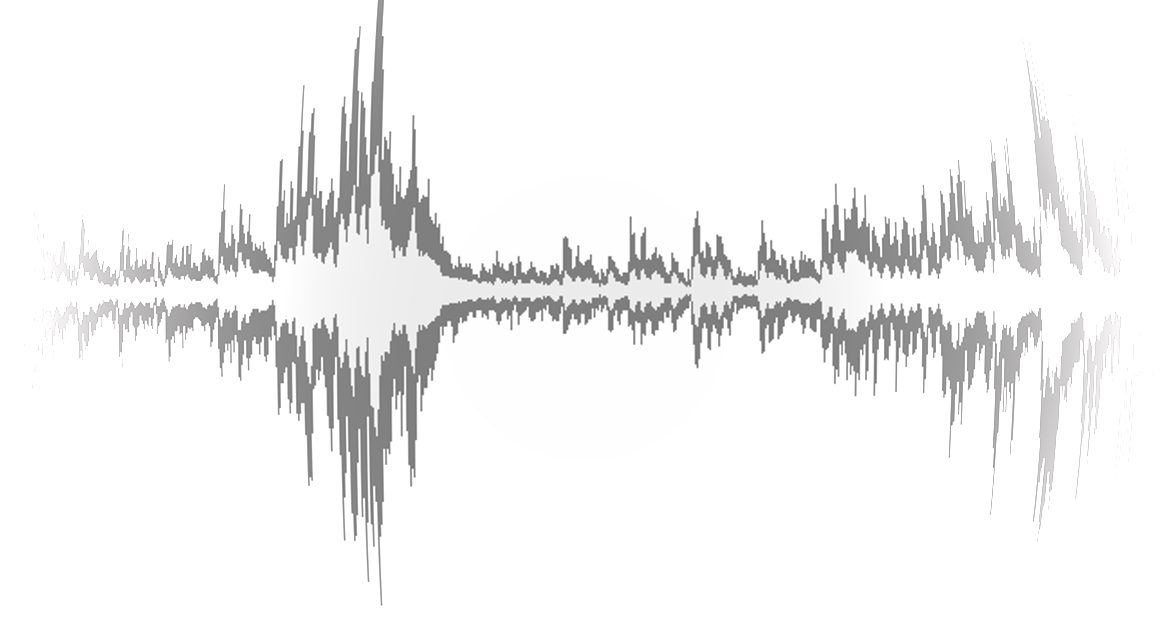
\includegraphics[width=\textwidth,height=3cm]{title}}


\begin{frame}
    \titlepage
    %\vspace{-5mm}
    \begin{flushright}
        \href{http://www.gtcmt.gatech.edu}{
\includegraphics[height=.8cm,keepaspectratio]{../shared/Logo_GTCMT_black}}
    \end{flushright}
\end{frame}


\section[intro]{introduction}
	\begin{frame}{real-time systems}{introduction}
        \begin{itemize}
            \item   many audio processing systems are real-time systems
            \item   this includes 
                \begin{itemize}
                    \item   most audio plugins, 
                    \item   studio hardware effects etc.
                \end{itemize}
        \end{itemize}
	\end{frame}

        \section{real-time systems}
	\begin{frame}{real-time systems}{introduction}
		\begin{block}{\textbf{real-time system} (wikipedia)}
            ``In a real-time digital signal processing (DSP) process, the analyzed (input) and generated (output) samples can be processed (or generated) continuously in the time it takes to input and output the same set of samples independent of the processing delay''
			
		\end{block}
        \pause
        \begin{itemize}
            \item   ``processing delay and resources must be bounded even if the processing continues for an unlimited time''
            \pause  
            \item   ``mean processing time per sample is no greater than the sampling period, which is the reciprocal of the sampling rate''
            \pause
            \item[$\Rightarrow$] ``perform all computations continuously at a fast enough rate that the output (...) keeps up with changes in the input signal'' 
        \end{itemize}
        
	\end{frame}

	\begin{frame}{real-time systems}{environment}
		\begin{itemize}
			\item	digital audio playback/recording: \textbf{constant stream} of audio samples to/from your sound device
				\begin{itemize}
					\item	distance of samples is defined by (constant!) sample rate
					\item \textbf{hard timing} --- no room for pauses
				\end{itemize}
			\item	if sound device (e.g., DAC) does not receive a sample in time, \textbf{audio will glitch}
			\bigskip
			\item<2-> typical operating systems work with \textbf{blocks of samples}
			\item<2-> typically, audio API \textbf{(quasi-)periodically} requests a block of samples	
		\end{itemize}
	\end{frame}
	
	\begin{frame}{real-time systems}{properties}
		\begin{itemize}
			\item	\textbf{performance}:
				\begin{itemize}
					\item	processing time for one block $\leq$ block length
                    \pause
                    \item   real-time computing does not necessarily mean high performance computing!
				\end{itemize}
			\bigskip
            \pause
			\item	\textbf{causality}:
				\begin{itemize}
                    \item   system output/state depends only on current and prior values
					\item	\textit{no} knowledge of future samples
				\end{itemize}
			\bigskip
			\pause
			\item	\textbf{latency}:
				\begin{itemize}
					\item	delay of a system between the stimulus and the response to
this stimulus
						\begin{itemize}
							\item	\textit{algorithmic delay}: (FFT-Processing, Look-Ahead, \ldots)
							\item	\textit{interface delay}: (block length, ad/da conversion)
						\end{itemize}
				\end{itemize}

		\end{itemize}
	\end{frame}

	\begin{frame}{real-time systems}{examples}
		\question{which of the following effects/processors are capable of real-time processing}
        \only<2>{
		\begin{itemize}
			\item	level normalization (normalize highest amplitude to max)
			\item	biquad EQ
			\item	reverb
			\item	pitch shifting
			\item	time stretching
		\end{itemize}
        }
        \only<3>{
		\begin{itemize}
			\item[--]	level normalization (normalize highest amplitude to max)
			\item[+]	biquad EQ
			\item[+]	reverb
			\item[+]	pitch shifting
			\item[--]	time stretching
		\end{itemize}
        }
	\end{frame}

	\begin{frame}{real-time systems}{clock}
        \begin{itemize}
            \item   \textbf{synchronization}
                \begin{itemize}
                    \item different components of a real-time systems have to be synchronized to work together
                    \item<2->[$\Rightarrow$] \textbf{master clock}
                    \smallskip
                    \item<3-> otherwise: multiple clocks have slight deviations and run out of sync ($\rightarrow$ buffer overflow/underflow $\rightarrow$ clicks)
                \end{itemize}
            
            \bigskip
            \item<4->   \textbf{master clock}
                \begin{itemize}
                    \item   on a computer: usually the sound card
                    \item   timers etc. that are not based on the sound card clock will \textbf{never} work
                \end{itemize}
           \end{itemize}
	\end{frame}
    
    
    \section{blocking}
   \begin{frame}{real-time systems}{blocking}
        \vspace{-3mm}
        \begin{itemize}
            \item \textbf{operating system/sound device}
                \begin{itemize}
                    \item   block size settings depend on \textit{latency and interactivity requirements}
                    \item   modern driver models and systems can achieve \textit{block sizes down to a few samples} at typical audio sample rates (that is not necessarily true for mobile devices)
                    \item   for some drivers the block size can vary
                    \item   \textit{typical range}: 32 -- 4096 samples, higher on Android
                    \item   despite the block size setting, there \textit{might be additional buffering} taking place in one of the layers between hardware and audio software
                \end{itemize}
            \smallskip
            \item<2->   \textbf{plugin host}
                \begin{itemize}
                    \item   often: simply the system block size for efficiency reasons
                    \item   but: block sizes \textit{may} vary (cf. automation)
                \end{itemize}
            \smallskip
            \item<3->   \textbf{plugin}
                \begin{itemize}
                    \item   needs to process/buffer \textit{any} input/output block size
                    \item   is likely to use a different block size and overlapping blocks internally (beware of workload peaks!)
                \end{itemize}
        \end{itemize}
    \end{frame}

	\begin{frame}{real-time systems}{block based processing}
		processing of \textit{blocks of samples} vs.\ individual samples
		
		\begin{figure}
			\centering
			\begin{footnotesize}
				\begin{picture}(60,40)
					\setcounter{iXOffset}{0}
					\setcounter{iYOffset}{24}
					\setcounter{iXBlockSize}{16}
					\setcounter{iYBlockSize}{4}
					\setcounter{iYBlockSizeDiv2}{2}
					\setcounter{iDistance}{8}

					% block indices
					\put(\value{iXOffset}, \value{iYOffset})
						{\text{{\shortstack[c]{$n$}}}}
					\addtocounter{iYOffset}{-\value{iYBlockSize}}
					\addtocounter{iYOffset}{-\value{iYBlockSizeDiv2}}
					\put(\value{iXOffset}, \value{iYOffset})
						{\text{{\shortstack[c]{$n+1$}}}}
					\addtocounter{iYOffset}{-\value{iYBlockSize}}
					\addtocounter{iYOffset}{-\value{iYBlockSizeDiv2}}
					\put(\value{iXOffset}, \value{iYOffset})
						{\text{{\shortstack[c]{$n+2$}}}}
					\addtocounter{iYOffset}{-\value{iYBlockSize}}
					\addtocounter{iYOffset}{-\value{iYBlockSizeDiv2}}
					\put(\value{iXOffset}, \value{iYOffset})
						{\text{{\shortstack[c]{$n+3$}}}}

					% audio time line
					\setcounter{iYOffset}{30}
					\setcounter{iXOffset}{5}
					\put(\value{iXOffset}, \value{iYOffset})
						{\vector(1,0){50}}
	
					% blocks
					\addtocounter{iXOffset}{5}
					\addtocounter{iYOffset}{-\value{iYBlockSize}}
					\addtocounter{iYOffset}{-\value{iYBlockSizeDiv2}}
					\put(\value{iXOffset}, \value{iYOffset})
						{\framebox(\value{iXBlockSize}, \value{iYBlockSize})}
					\addtocounter{iXOffset}{5}
					\addtocounter{iYOffset}{-\value{iYBlockSize}}
					\addtocounter{iYOffset}{-\value{iYBlockSizeDiv2}}
					\put(\value{iXOffset}, \value{iYOffset})
						{\framebox(\value{iXBlockSize}, \value{iYBlockSize})}
					\addtocounter{iXOffset}{5}
					\addtocounter{iYOffset}{-\value{iYBlockSize}}
					\addtocounter{iYOffset}{-\value{iYBlockSizeDiv2}}
					\put(\value{iXOffset}, \value{iYOffset})
						{\framebox(\value{iXBlockSize}, \value{iYBlockSize})}
					\addtocounter{iXOffset}{5}
					\addtocounter{iYOffset}{-\value{iYBlockSize}}
					\addtocounter{iYOffset}{-\value{iYBlockSizeDiv2}}
					\put(\value{iXOffset}, \value{iYOffset})
						{\framebox(\value{iXBlockSize}, \value{iYBlockSize})}

	
					% lengths
					\linethickness{.03mm}
					\setcounter{iYOffset}{34}
					\setcounter{iXOffset}{10}
					\put(\value{iXOffset}, \value{iYOffset})
						{\line(0,-1){12}}
					\put(\value{iXOffset}, \value{iYOffset})
						{\vector(1,0){1}}
					\addtocounter{iXOffset}{5}
					\put(\value{iXOffset}, \value{iYOffset})
						{\line(0,-1){18}}
					\put(\value{iXOffset}, \value{iYOffset})
						{\vector(-1,0){1}}
					\addtocounter{iXOffset}{5}
					\addtocounter{iXOffset}{5}
					\put(\value{iXOffset}, \value{iYOffset})
						{\line(0,-1){30}}
					\put(\value{iXOffset}, \value{iYOffset})
						{\vector(1,0){1}}
					\addtocounter{iXOffset}{\value{iXBlockSize}}
					\put(\value{iXOffset}, \value{iYOffset})
						{\line(0,-1){30}}
					\put(\value{iXOffset}, \value{iYOffset})
						{\vector(-1,0){1}}

					\put(11, 34)
						{\text{$\mathcal{H}$}}
					\put(32, 34)
						{\text{$\mathcal{K}$}}
					\put(56, 28)
						{\text{$i$}}
				\end{picture}
\end{footnotesize}

		\end{figure}
		\pause
		\vspace{-5mm}
		\textbf{reasons}:
		\begin{itemize}
			\item	block based algorithms (FFT, \ldots)
			\item	audio hardware characteristics
			\item	efficiency (SIMD, memory allocation)
		\end{itemize}
	\end{frame}
    %\begin{frame}{real-time systems}{block sizes}
        %\begin{itemize}
            %\item   typical block sizes can range from 1\ldots thousands of samples
            %\item   often powers of 2
            %\bigskip
            %\item<2->   in many DAWs and some drivers the \textbf{block size varies}
        %\end{itemize}
    %\end{frame}
 		

	\begin{frame}{real-time systems}{blocking}
        \vspace{-3mm}
        \begin{itemize}
            \item   \textbf{time-stamps}
                \begin{itemize}
                    \item   blocking can be considered similar to down-sampling
                    \item[$\Rightarrow$]   \textit{what time stamps to assign to each block?}
                        \begin{itemize}
                            \item   begin of each block
                            \item   center of each block
                        \end{itemize}
                \end{itemize}
            \bigskip
            \item<2->   \textbf{initialization}
                \begin{itemize}
                    \item   real-time systems are designed to work for infinite input stream
                    \item[$\Rightarrow$]   \textit{how to initialize internal buffers?}
                        \begin{itemize}
                            \item   usually zeros, but other initializations may make sense in specific scenarios
                        \end{itemize}
                \end{itemize}
            \bigskip
            \item<3->   \textbf{performance} issues due to blocking
                \begin{itemize}
                    \item   plugin gets stream of samples split into small blocks (e.g., 32 samples)
                    \item   internally, STFT with large hopsize (e.g., 2048 samples) is used 
                    \item[$\Rightarrow$]   \textit{what is the potential performance problem here?}
                        \begin{itemize}
                            \item<4->   each hop requires data from 64 input blocks
                            \item<4->[$\Rightarrow$]   no processing can be done for 63 blocks
                            \item<4->[$\Rightarrow$]   processing of huge FFT has to be done during the 64th block (32 samples)
                        \end{itemize}
                \end{itemize}
       \end{itemize}
    \end{frame}
    
    \begin{frame}{real-time systems}{inplace processing}
        \question{what is ``inplace processing''}
        
        \bigskip
        
        \begin{itemize}
            \item   samples of the input block are replaced with the output block
                \begin{itemize}
                    \item<3->[$+$]  resource friendly: memory allocation for output buffer
                    \item<3->[--]  original input data cannot be used anymore
                \end{itemize}
        \end{itemize}
    \end{frame}

\section{summary}
		\begin{frame}{summary}{real-time systems}
            real-time systems have the following properties:
            \smallskip
            \begin{itemize}
                \item   hard \textbf{performance} requirements
                    \begin{itemize}
                        \item   processing of input block has to be faster then time span of this block \textbf{for each block, not only on average}
                    \end{itemize}
                \smallskip
                \item   \textbf{causality}
                    \begin{itemize}
                        \item   future samples cannot taken into account (or only by increasing the latency: look-ahead)
                    \end{itemize}
                \smallskip
                \item   \textbf{latency}
                     \begin{itemize}
                        \item   time between input and system response, usually intended to be minimal
                    \end{itemize}
           \end{itemize}
 		\end{frame}

\end{document}

